% Aquí van todos los diagramas UML
\usepackage{tikz-uml}

% Diagrama de clases
\newcommand{\clases}{
\begin{figure}
\centering
\begin{tikzpicture}

% Clase Pizarra
\umlclass{Pizarra}{
  - estado : Estado \\ 
  - usuarios : ArrayList$<$Usuario$>$\\
  - estadisticas : ArrayList$<$Estadisticas$>$\\
  - niveles : ArrayList$<$Nivel$>$\\
  - conf : Configuracion\\
}{ 
  + mostrarEstadisticas(String userid, Usuario user):String\\
  + mostrarEstadisticasGenerales(Usuario user):String\\
  + escribir(String direccion, Archivo archivo, Usuario user)\\
  + leer(String direccion, Usuario user):Archivo\\
  + escrituraLectura(String direccion, Archivo archivo, Usuario user): Archivo\\
  + mostrarEstado(Usuario user):Usuario\\
  + buscar(String nombre, Usuario user):Estado\\
  + comparar(Archivo arch1, Archivo arch2, Usuario user):Archivo\\
  + crearCarpeta(String direccion, String nombre, Usuario user): Bool\\
  + crearUsuario(String nombre, String userid, String pass, Nivel nivel, Usuario user)\\
  + gestionarPermisos(Nivel nivel, Bool[] permisos, Usuario user): Bool\\
  + configurarPizarra(Configuracion config, Usuario user): Bool\\
  + getUsuario(String userid):Usuario\\
  - setEstado(Estado)\\
  - setUsuarios(ArrayList$<$Usuario$>$)\\
  - setEstadisticas(ArrayList$<$Estadisticas$>$)\\
  - comprobarPermisos(Usuario user, int permiso):Bool
}

% Clase Agente
\umlclass[x=0, y=-14]{Agente}{
  - userid : String\\
  - pass : String\\
  - pizarra : Pizarra\\
  - usuario : Usuario\\
}{
  + Agente(String userid)\\
  + Agente(Pizarra pizarra)\\
  + iniciarSesion(String userid, String pass):Bool\\
  + mostrarEstadisticas(String userid)\\
  + mostrarEstadisticasGenerales()\\
  + escribir(String direccion, Archivo archivo)\\
  + leer(String direccion):Archivo\\
  + escrituraLectura(String direccion, Archivo archivo):Archivo\\
  + mostrarEstado():Estado\\
  + buscar(String nombre):String\\
  + comparar(Archivo arch1, Archivo arch2):Archivo\\
  + crearCarpeta(String direccion, String nombre):Bool\\
  + crearUsuario(String nombre, String userid, String pass, Nivel nivel)\\
  + gestionarPermisos(Nivel nivel, Bool[] permisos): Bool\\
  + configurarPizarra(Configuracion config)\\
  + setUserid(String userid)\\
  + setPass(String pass)\\
  - comprobarPermisos(Usuario user, int permiso):Bool\\
  - establecerConexion(Pizarra pizarra)\\
  - cerrarSesion(Pizarra pizarra) 
}

% Clase Usuario
\umlclass[x=13, y=0]{Usuario}{
  - nombre : String\\
  - userid : String\\
  - pass : String\\
  - nivel : Nivel
}{
  + comprobarUser(String pass): Bool\\
  + getNombre() : String\\
  + getUserid() : String\\
  + getNivel() : Nivel\\
  + setPass(String pass)\\
  + setNivel(Nivel nivel) 
}

% Clase Estadisticas
\umlclass[x=13, y=8]{Estadisticas}{
  - userid : String\\
  - datos[] : Integer\\
}{
  + actualizarEstadisticas(datos[] int)\\
  + getUsuario() : String\\
  + getDatos() : Integer[]\\
}

% Clase Configuracion
\umlclass[x=4, y=9.5]{Configuracion}{
  - visibilidad : Bool\\
  - IP : String\\
  - puerto : int\\
  - maxConexion : int\\
  - espacio : int\\
  - maxUser : int\\
  - depuracion : Bool\\
}{
}

% Clase Estado
\umlclass[x=-6, y=10]{Estado}{
  - ArrayList$<$Elemento$>$
}{

}

% Clase Elemento
\umlclass[x=-15, y=10]{Elemento}{
   \# nombre : String
}{

}

% Clase Carpeta
\umlclass[x=-17, y=6]{Carpeta}{
   - ArrayList$<$Elemento$>$
}{

}

% Clase Archivo
\umlclass[x=-11, y=6]{Archivo}{

}{

}

% Clase Nivel
\umlclass[x=-13, y=0]{Nivel}{
   - permisos[\$NPermisos\$] : Bool
}{
   + cambiarPermiso(int permiso, estado Bool)\\
   + resetPermisos()\\
   + setPermisos()\\
   + getPermisos():Bool[]
}

% Nota de la clase Nivel
\umlnote[x=-13, y=-5, width=5cm]{Nivel}{\textbf{\$NPERMISOS\$} es la cantidad de opciones que puede tener la plataforma, siendo cada posición una de estas opaciones}

% Relaciones

\umlinherit[geometry=-|]{Carpeta}{Elemento}

\umlcompo[mult1=0..n, mult2=1]{Elemento}{Carpeta}

\umlinherit{Archivo}{Elemento}

\umlcompo[mult2=1, mult1=0..n]{Elemento}{Estado}

\umlimpl{Pizarra}{Nivel}

\umlimpl[geometry=-|]{Pizarra}{Estado}

\umlimpl[geometry=-|]{Pizarra}{Configuracion}

\umlimpl{Pizarra}{Estadisticas}

\umlimpl{Pizarra}{Usuario}

\umlimpl{Agente}{Pizarra}

\end{tikzpicture}
\end{figure}
}
